

\chapter{Conclusion}

At the beginning of the LHC physics program, there was much hope for the
resolution of a number of open issues in particle physics and the potential
discovery of a plethora of new particles.
In some ways, the first years of the LHC was an immense success.
The high energies and luminosities coupled with the incredibly powerful
and precise particle detectors led to measurements with incredible
accuracy.

\begin{figure}[ht!]
  \begin{center}
    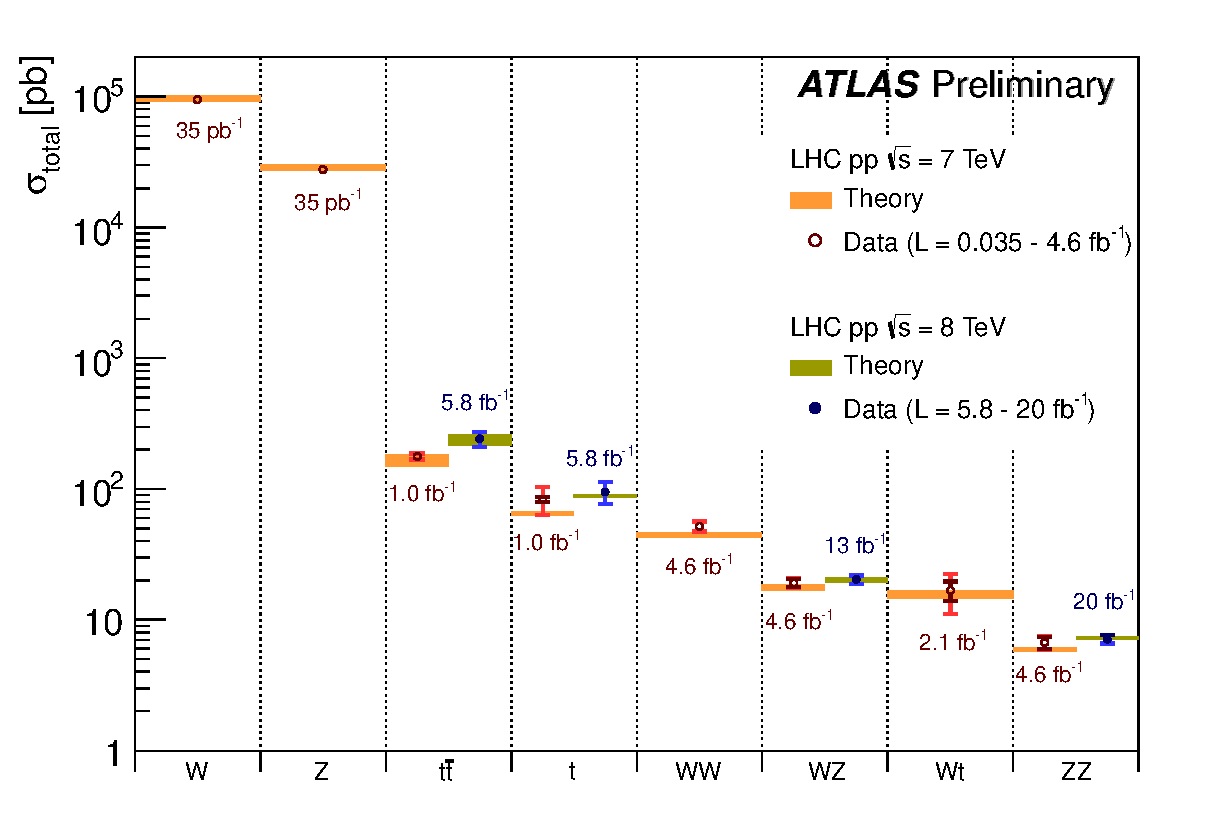
\includegraphics[width=.75\textwidth]{figures/conclusion/SM_SummaryPlotMoriondEWK2013}
    \caption{Measurements of the cross-sections of various particles of the Standard Model and comparisons to their theoretical predictions at $\sqrt{s}=7$ and $\sqrt{s} = 8$ TeV.}
    \label{fig:xsec_vs_roots}
  \end{center}
\end{figure}


Among these are many detailed studies of the top quark, which levered
advanced experimental and statistical techniques to achieve world class measurements.
This thesis described a number of analyses which resulted in world class measurements
of the top quark pair-production cross-section, including a statistical combination
of analyses that resulted in the most powerful measurement of the $\ttbar$ cross
section measured at the LHC at the time.

\begin{figure}[ht!]
  \begin{center}
    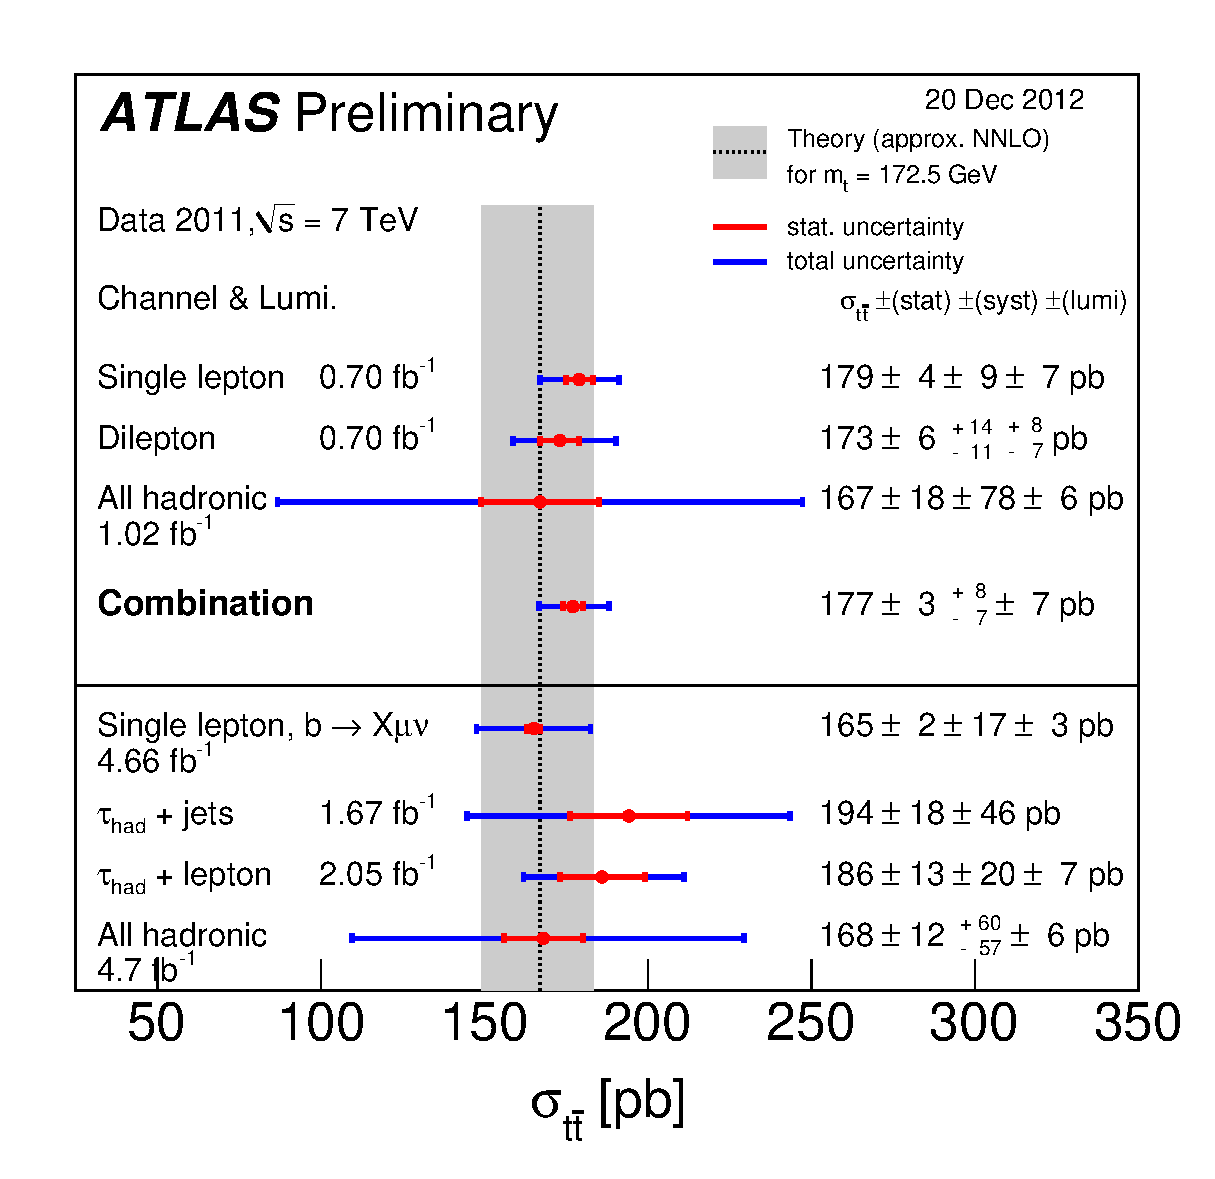
\includegraphics[width=.75\textwidth]{figures/conclusion/tt_xsec20Dec2012}
    \caption{Summary of measurements of the top quark cross-section, including the pair-production cross-section measurements presented in this thesis as well as measurements using hadronic tau decays.}
    \label{fig:xsec_vs_roots}
  \end{center}
\end{figure}
\clearpage

And chief among the successes of the early LHC program was the discovery of the Higgs boson\cite{HiggsObservation:2012}.
The discovery of the Higgs was a triumph for the Standard Model and a clear demonstration of the power of the ATLAS detector.
It demonstrated that a version of the Higgs mechanism is indeed the source of electroweak symmetry breaking in the Standard Model.
However, because only the version of the Higgs boson predicted by the Standard Model was found, the discovery didn't shed
any light on some of the important open questions in particle physics.

\begin{figure}[ht!]
  \begin{center}
    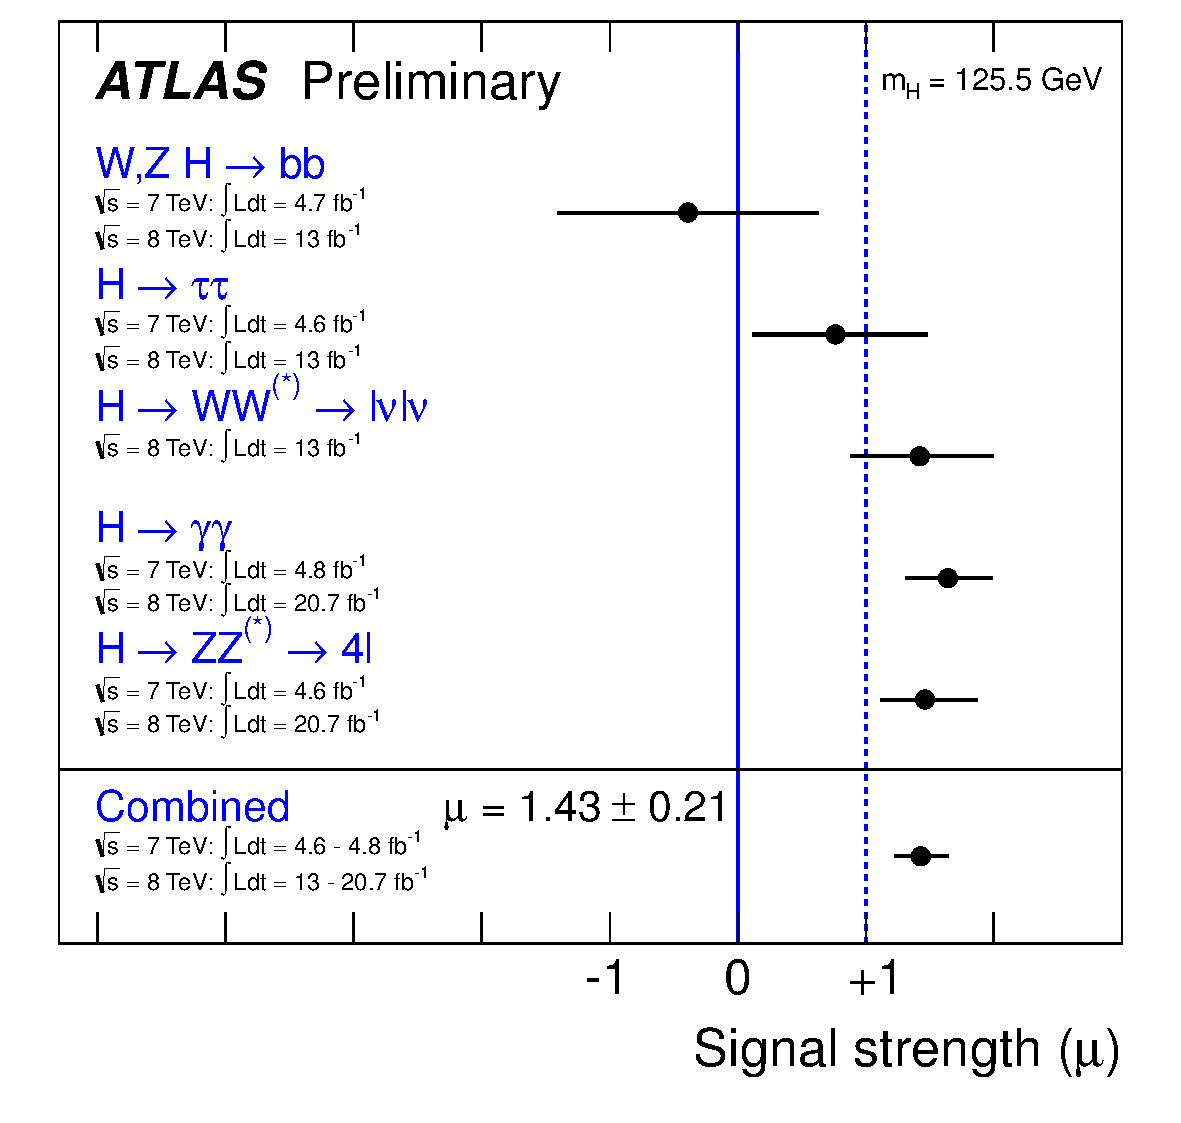
\includegraphics[width=.75\textwidth]{figures/conclusion/HiggsCrossSection}
    \caption{Summary of measurements of the cross-section of the Higgs boson using various decay channels.
      The signal strength, $\mu$, is the ratio of the measured cross-section to the theoretical value, assuming a higgs mass of 125.5 GeV.}
    \label{fig:higgs_cross_section}
  \end{center}
\end{figure}
\clearpage

However, motivated by the hierarchy problem, many had hoped that the mechanism of electroweak
symmetry breaking would be more rich than the Higgs mechanism of the Standard Model and
would bring with it a number of new particles.
Many believed that the discovery of Super Symmetric partners would shed light on the
Hierarchy Probloem and would lead to a more natural understanding of electroweak symmetry breaking.
However, extensive studies on numerous supersymmetric models have yet to find evidence
supporting the existence of supersymmetric partners.
In addition to spectrum of Supersymmetric models, the experiments at the LHC have searched
for more exotic physical models, many of which were theorized to address the hierarchy
problem and other shortcomings of the Standard Model.

\begin{figure}[ht!]
  \begin{center}
    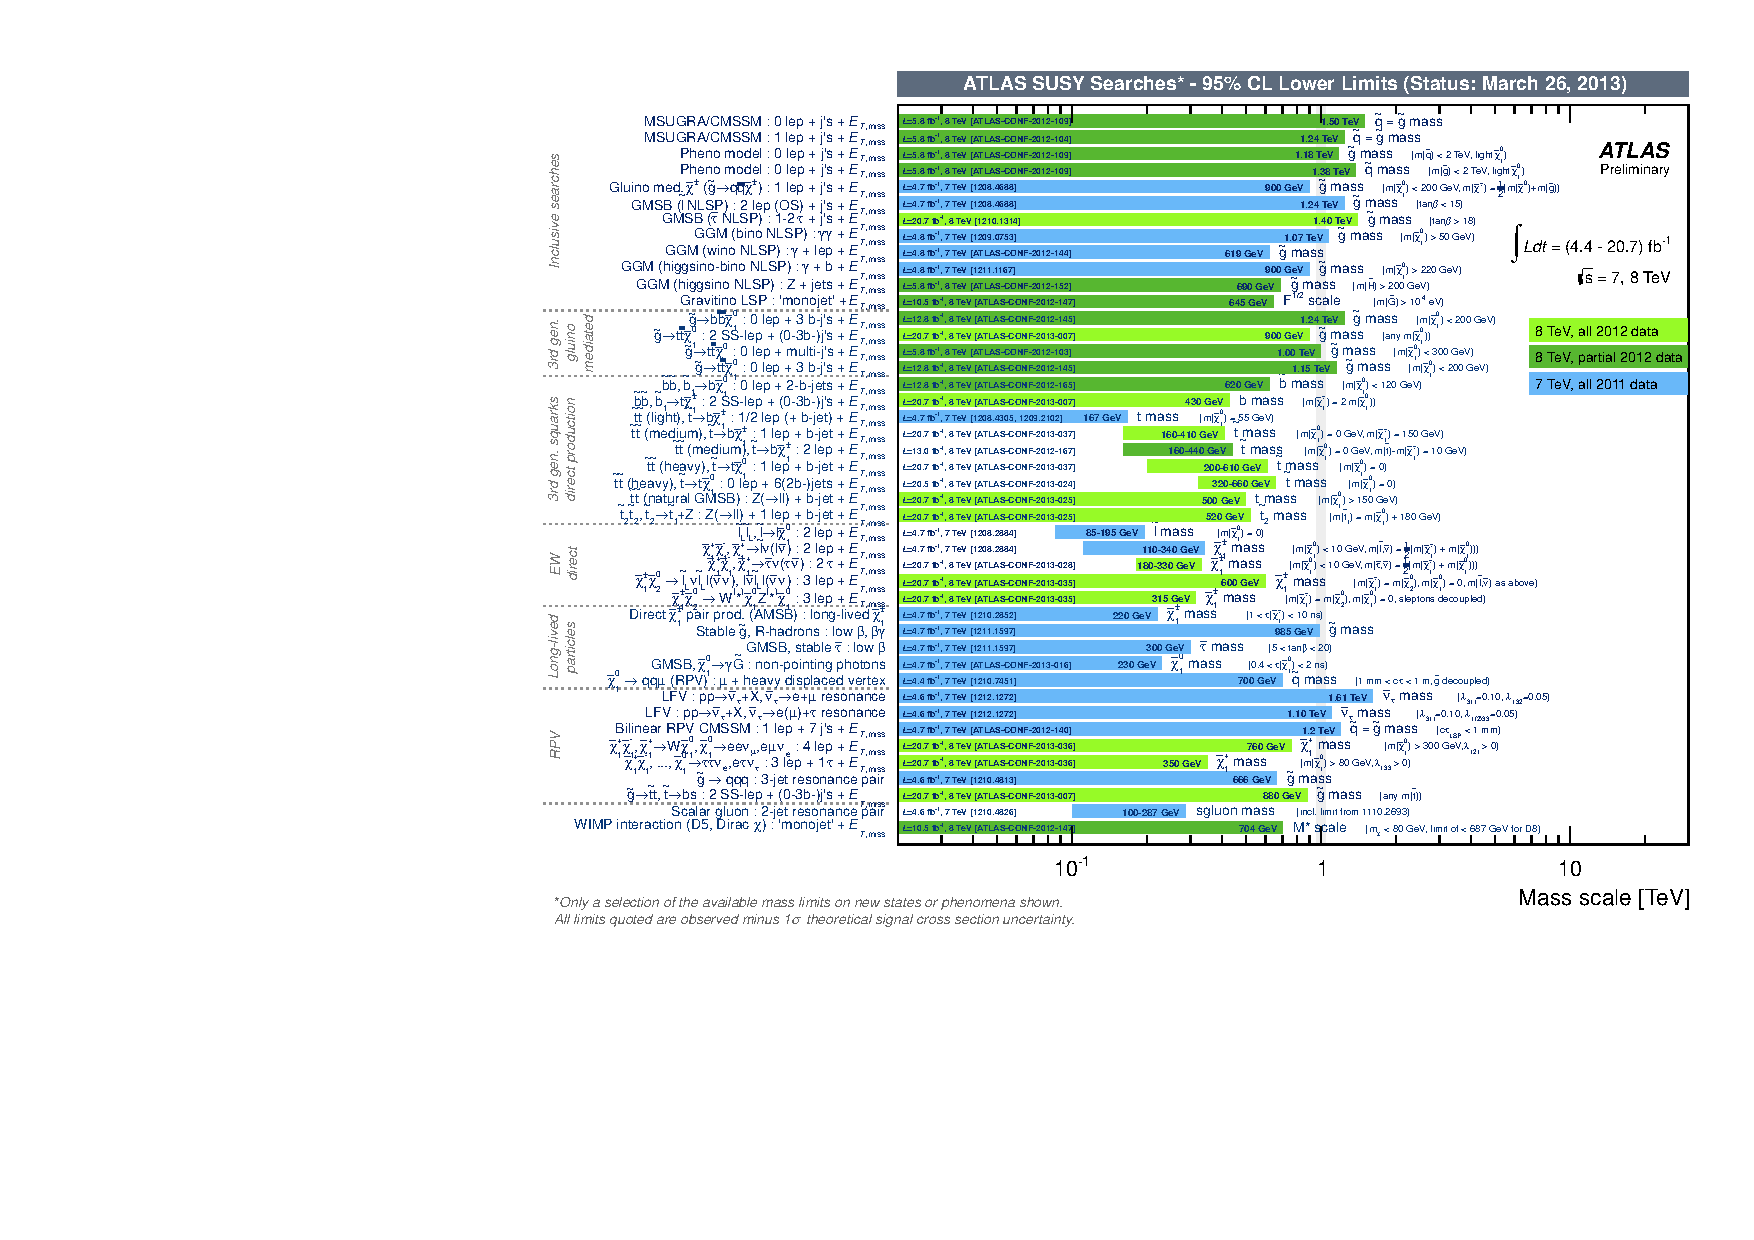
\includegraphics[width=.75\textwidth]{figures/conclusion/Susy}
    \caption{Limits on Super Symmetric parameters and particles obtained using the ATLAS detector at a center-of-mass energy of $\sqrt{s}=7$ and $\sqrt{s} = 8$ TeV.}
    \label{fig:susy}
  \end{center}
\end{figure}


\begin{figure}[ht!]
  \begin{center}
    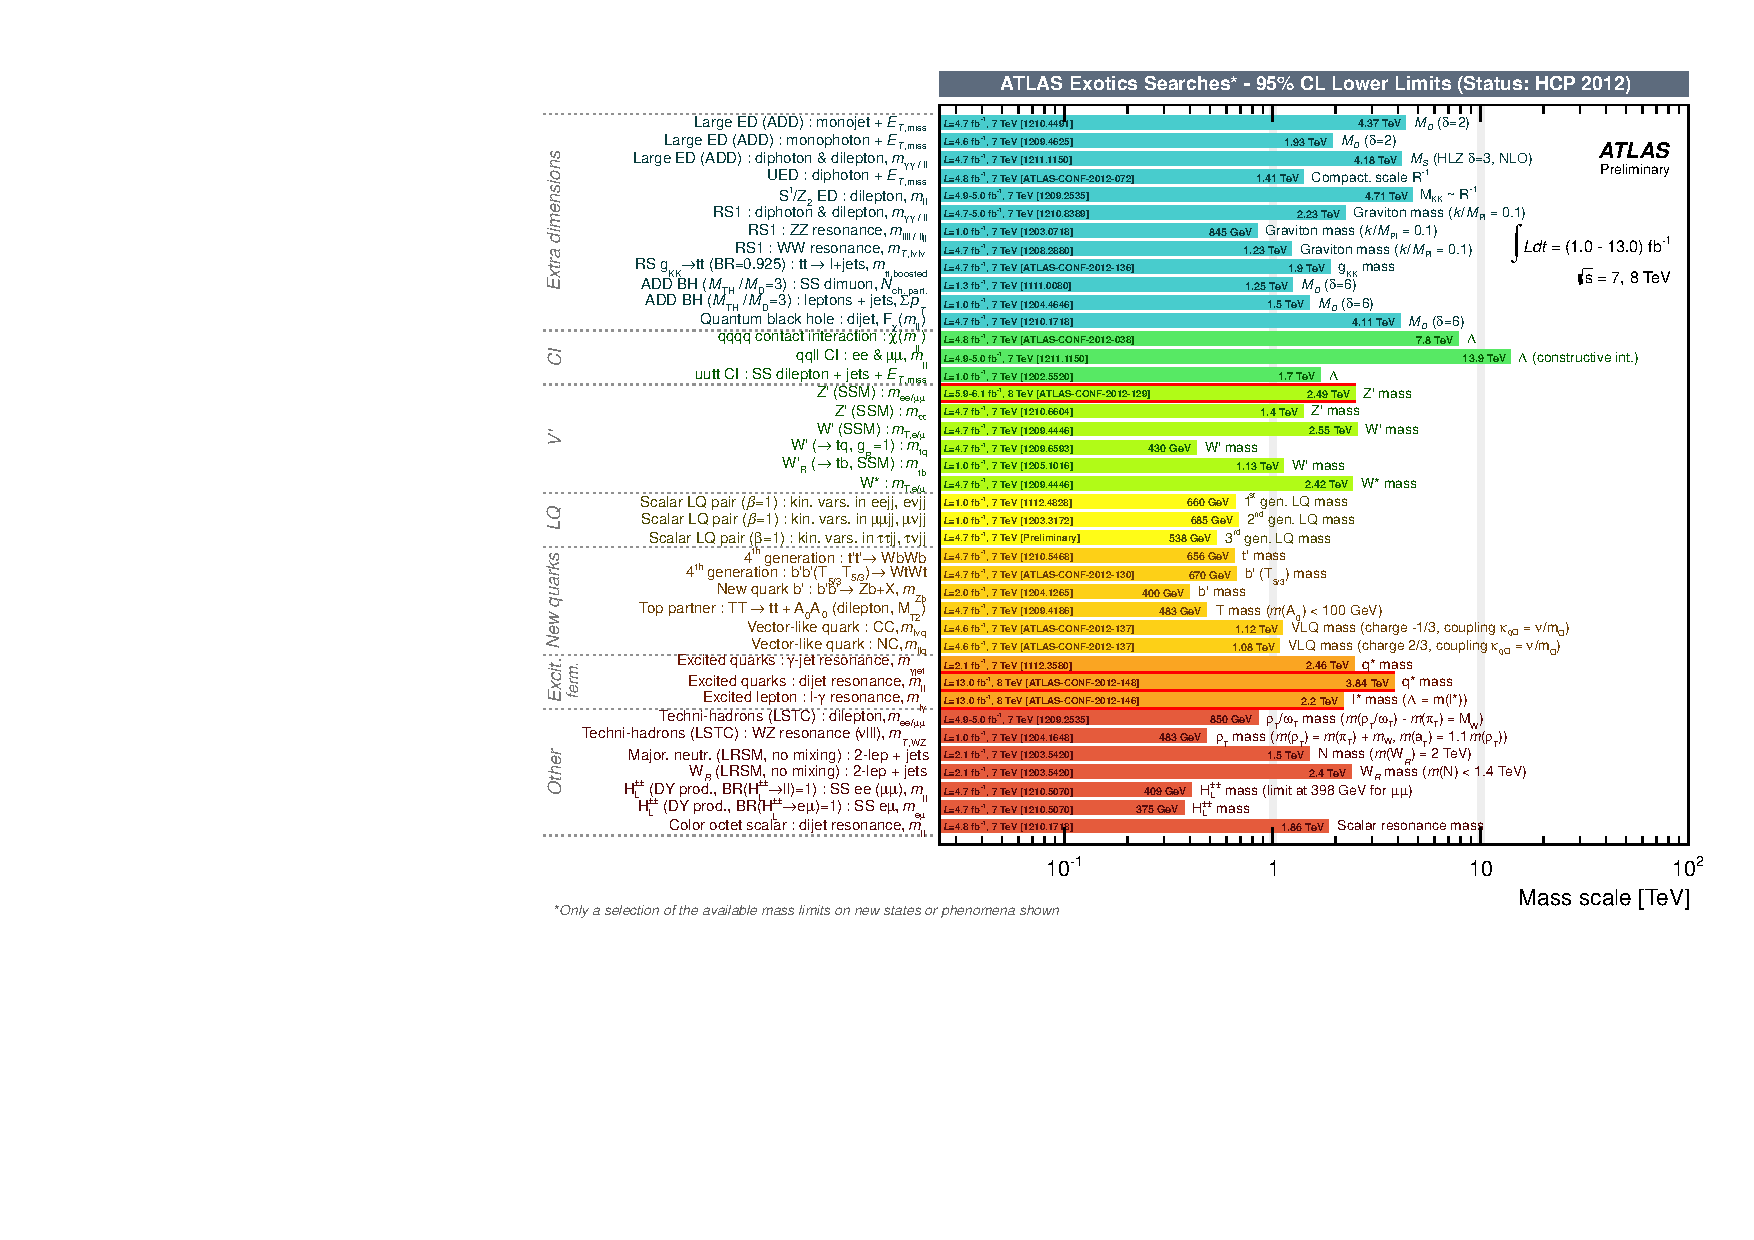
\includegraphics[width=.75\textwidth]{figures/conclusion/ExoticResultsSummary}
    \caption{Measured limits on the properties of various exotic particles proposed by extensions to the Standard Model. The limits shown were made using data obtained at center-of-mass-energies of $\sqrt{s}=7$ and $\sqrt{s} = 8$ TeV.}
    \label{fig:xsec_vs_roots}
  \end{center}
\end{figure}

This thesis described a search for exotic processes in the same-sign dilepton plus jets signature that
was aimed at discovering a number of potential particles, including particles from models that provide
exotic explanations of the hierarchy problem.
However, no evidence supporting these models was found in the data.

The lack of evidence for new physics at the electroweak scale suggests a number of possible conclusions.
While the LHC has extensively searched the for new physics using center-of-mass energies of $\sqrt{s}=7$ and $\sqrt{s} = 8$ TeV,
it could be the case that new physics addressing the hierarchy problem is still beyond the reach
of the LHC (but not so out of reach to be unnatural).
Or perhaps the arguments insisting on a natural theory of fundamental particle physics are ill founded.
